\chapter{TC4合金固溶时效处理}

本设计中对于$\alpha+\beta$型的\ti 钛合金,采用了固溶+时效热处理来进行强化,设置的主要参数为固溶温度、冷却速度、时效温度\cite{mirror1,ranxingGurongwenduduiTi6Al4VELItaihejinxianweizuzhijixingnengdeyingxiang2021}。其中固溶处理的目的是为了使合金元素在高温状态下充分扩散,从而通过$\alpha \to \beta$相变来获得亚稳定相(如$\alpha^{\prime}$相、$\alpha^{\prime\prime}$相以及$\beta^{\prime}$相等)以改善组织的形貌,而同时不稳定的亚稳相也能为时效处理提供组织基础。时效处理的目的则是在固溶处理后使组织中的亚稳定相向稳定状态转变,通过二次相变的析出相来改善合金的力学性能,比如促进针状$\alpha^\prime$马氏体的分解以提高塑性等。

\ti 合金热处理中,$\beta$相变点温度是区分不同热处理工艺强化效果的一把重要标尺。固溶温度的不同会使$\alpha$相转化成不同含量的$\beta$相组织,进而导致高温$\beta$相在冷却过程中生成了不同的亚稳相。本章通过对力学拉伸试验的数据与热处理工艺参数进行了正交对比分析,得到了影响力学性能的主次要因素,研究了组织的形貌特点、力学性能同固溶温度、冷却方式、时效温度三者之间的关系。
\section{实验数据分析}
\subsection{力学性能分析}
通过对万能力学试验机上测试得到的数据进行整理,去除了力学拉伸曲线中断裂瞬间到试验结束之间的无用值,对屈服强度不明显的拉伸曲线进行拟合、求交,并对各组两个式样的实验数据进行平均化处理,整合汇总得到了如\ref{sec:mystrength}的结果:%\footnote{根据《金属材料室温拉伸试验方法》GBT228-2002,抗拉强度符号已经由$ R_m $代替旧国标中的$ \sigma_b $,故在此使用最新标准$ R_m $来表示抗拉强度。}
\begin{table}[htbp]
	\centering
		\zihao{5}
	\caption{\ti 合金的力学性能试验结果}
	\label{sec:mystrength}
	\begin{tabular}{ccccc}
		\toprule
		试验编号& 代号&$ R_m $(MPa)&$ R_{0.2} $(MPa)&延伸率 \\
		\midrule
		0 & 甲 & 1008.69 &986.32& 6.83$\%$ \\
		1 & 乙 & 1188.36 &1054.61 &3.73$\%$ \\
		2 & 丙 & 1077.33 & 997.07&4.24$\%$ \\
		3 & 丁 & 1094.87 & 998.00&3.49$\%$ \\
		4 & 戊 & 1099.33 &986.20 &2.60$\%$ \\
		5 & 己 & 1113.90 & 1021.35&2.57$\%$ \\
		6 & 庚 & 1077.28 &992.31& 2.88$\%$ \\
		7 & 辛 & 790.10 & 脆断&1.94$\%$ \\
		8 & 壬 & 799.54 &脆断& 2.05$\%$ \\
		9 & 癸 & 873.38 & 脆断&2.19$\%$ \\
		\bottomrule
	\end{tabular}
\end{table}

通过在室温力学拉伸试验,得到了试样断裂区域截面($ 1.3mm\times2.5mm=3.25mm^2 $)的应力与应变曲线(拉伸变形量与拉伸区域长度的比值),再将把包括未处理的对照组在内的十组数据的应力应变曲线进行汇总,得到了如\ref{fig:试样应力应变曲线汇总}\footnote{图形中标签未标明的,所有组共同具有工艺参数为:固溶处理时间60分钟;时效处理时间60分钟}所示的应力应变曲线汇总图:
\begin{figure}[h!]
	\centering
	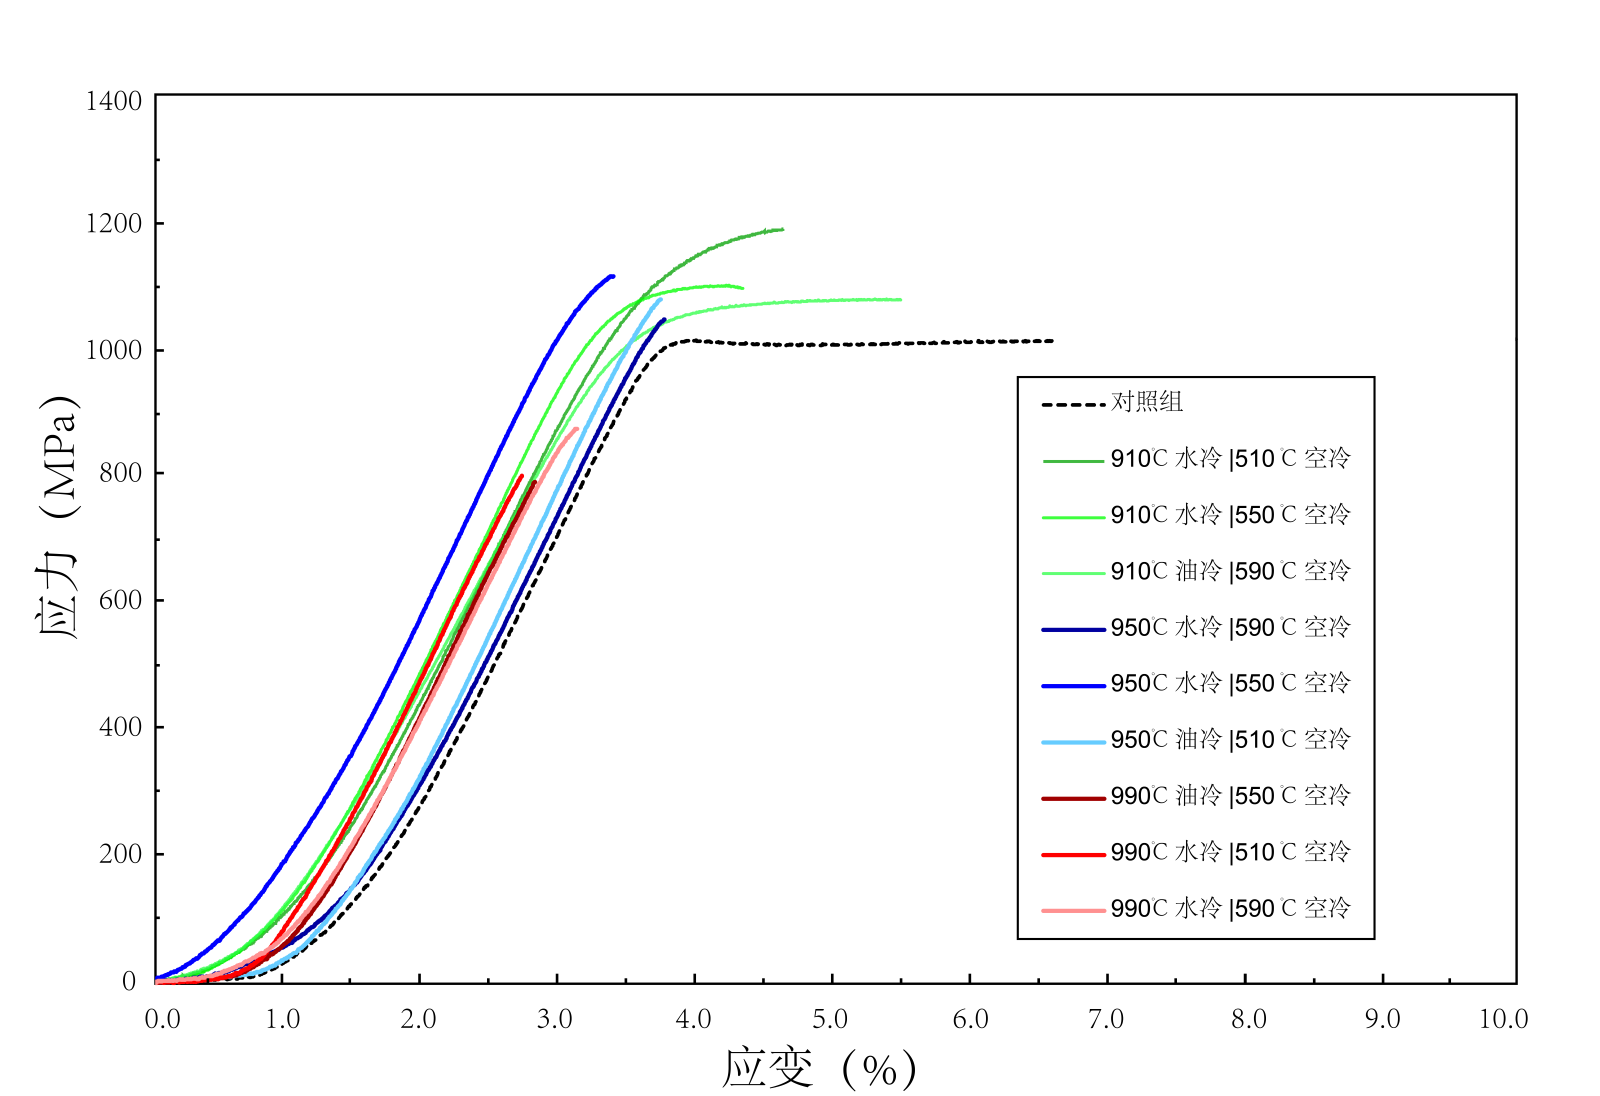
\includegraphics[width=0.99\linewidth]{pic/试样应力应变曲线汇总min.png}
	\caption{试样应力应变曲线汇总}
	\label{fig:试样应力应变曲线汇总}
\end{figure}


从图中经过分析可以看出:固溶-时效处理后试样对材料各方面的影响还是比较明显的,经过不同参数的热处理后,有如下力学性能特点:
\begin{enumerate}
	\item {整体塑性降低:}与对照组相比,热处理后的合金塑性均大幅度降低,910℃固溶处理后的三组在经过短暂的屈服后即被拉断,而950℃、990℃固溶处理后的六组则几乎呈现出来脆性材料的特点,断裂都属于脆性断裂\footnote{除了组织形貌外,拉伸试验时速率过大也有可能导致合金发生了脆断}。
	\item {抗拉强度有所提升:}910℃、950℃固溶组的抗拉强度与对照组相比都有所提升,其中以910℃固溶水冷+510℃时效空冷组的强度为最高。
	\item {固溶温度大于$\beta$相变点时,强度显著降低。}990℃固溶处理三组试样的各项力学性能指标明显下降,其中990℃固溶油冷+550℃时效空冷组的抗拉强度已经降低到了$ 790MPa $左右,990℃固溶水冷+510℃时效空冷组的最大应变才达到$ 2.18\% $,仅仅是对照组$ 6.83\% $的三分之一。
\end{enumerate}
\subsection{正交实验设计分析}
本设计通过正交实验饭进行实验的设计,通过正交实验法得到的固溶温度、冷却方式、时效温度与力学性能之间的关系如下:
\begin{table}[htbp]
	\centering
		\zihao{5}
	\caption{固溶温度、冷却方式、时效温度与抗拉强度关系表}
	\label{sec:zjq}
	\begin{tabular}{cccccc}
		\toprule
		差异源 & 平方和 & 自由度 & 均方 & $ F_1 $ & $ p_1 $ \\
		\midrule
		截距 & 8078602.799 & 1 & 8078602.799 & 3561.305 & 0.009 \\
		固溶温度 & 166133.961 & 2 & 83066.98 & 36.619 & 0.008 \\
		冷却方式 & 4354.254 & 1 & 4354.254 & 1.919 & 0.26 \\
		时效温度 & 804.901 & 2 & 402.45 & 0.177 & 0.846 \\
		%Residual & 6805.317 & 3 & 2268.439
		\bottomrule
	\end{tabular}
\end{table}
\begin{table}[htbp]
	\centering
		\zihao{5}
	\caption{固溶温度、冷却方式、时效温度与延伸率关系表}
	\label{sec:zjy}
	\begin{tabular}{cccccc}
		\toprule
		差异源 & 平方和 & 自由度 & 均方 & $ F_2 $ & $ p_2 $ \\
		\midrule
		截距 & 0.007 & 1 & 0.007 & 2565.824 & 0.004 \\
		固溶温度 & 0 & 2 & 0 & 91.373 & 0.002 \\
		冷却方式 & 0 & 1 & 0 & 4.717 & 0.118 \\
		时效温度 & 0 & 2 & 0 & 3.471 & 0.166 \\
		\bottomrule
	\end{tabular}
\end{table}

利用三因素方差分析去研究固溶温度,冷却方式和时效温度对于抗拉强度和延伸率的影响关系,从\ref{sec:zjq}和\ref{sec:zjy}可以看出:固溶温度对两者的影响呈现出显著性($ F_{1固} =36.619,p_{1固}=0.008< 0.05 $、$ F_{2固} =91.373,p_{2固}=0.002< 0.05 $) ,说明主效应存在,固溶温度会对抗拉强度和延伸率产生差异关系。冷却方式没有呈现出显著性($ F_{1冷}=1.919,p_{1冷} =0.260>0.05 $、$ F_{2冷}=4.717,p_{2冷}=0.118>0.05 $) ,说明冷却方式并不会对抗拉强度产生差异关系。时效温度没有呈现出显著性($ F_{1时}=0.177,p_{1时}=0.846>0.05 $、$ F_{2时}=3.471,p_{2时} =0.166>0.05 $) ,说明时效温度并不会对抗拉强度产生差异关系。可见固溶温度对试样力学性能的影响最大,冷却方式与固溶温度的影响都较小,尤以固溶温度的影响为最小。

\subsection{组织转变机理分析}
本设计设置的固溶温度在相变点附近,采用两个冷却速度不同的方式进行淬火,在高温状态下进行保温目的是为了使合金内部化学元素间产生的充分弥散,使成分均匀化,并发生 $\alpha\to\beta$ 转变以获得高温$ \beta $相组织。


保温一段时间后,在较快冷却条件下抑制钛合金自发的$\beta\to \alpha$ 转变, 从而获得亚稳$ \beta^{\prime} $相,以便于通过时效处理使组织强化。组织转变图如\ref{fig: micchange}所示\cite{YangJingJingJiGuangXuanQuRongHuaChengXingTi6Al4VHeJinDeZuZhiYanBianJiDiaoKong2017a}
%TC4 钛合金在稳定状态下含有少量的 $\beta$ 相,$\beta$ 相的存在使其具有热处理强化的能 力。由\ref{fig:tc4change}可知,固溶处理过程中固溶温度对固溶后的亚稳定相种类起决定作 用,不同固溶温度下 $\alpha$ 与 $\beta$ 相的平衡体积分数不同,造成 $\beta$ 相中合金元素含量不同, 从而在快速冷却过程中产生不同的亚稳定相。


\begin{figure}[h!]
	\centering
	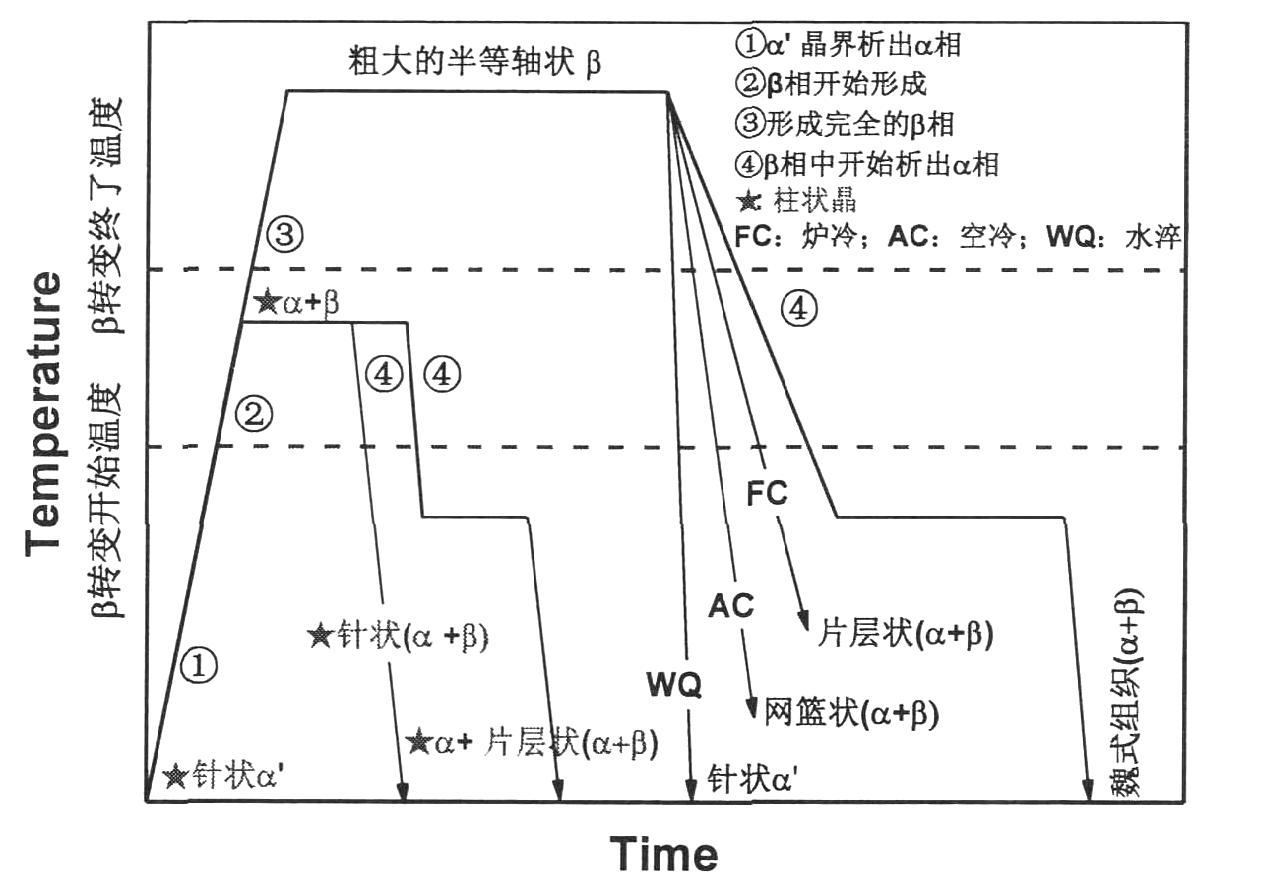
\includegraphics[width=0.7\linewidth]{pic/组织转变图}
	\caption{组织转变图}
	\label{fig: micchange}
\end{figure}

%\begin{figure}[h!]
%	\centering
%	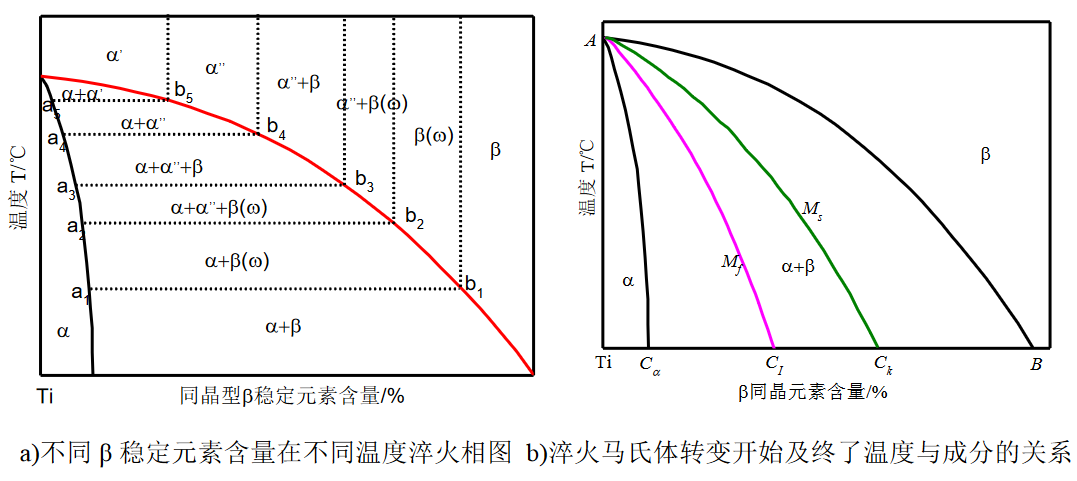
\includegraphics[width=0.7\linewidth]{pic/tc4change}
%	\caption{钛合金在淬火过程中的亚稳定相及马氏体转变温度}
%	\label{fig:tc4change}
%\end{figure}

%固溶处理得到的组织可以为后续的时效处理提供良好的组织状态。本实验时效处理的温度较低,在500℃附近,通过将固溶处理后得到的亚稳态组织加热到一定温度后保温60分钟,目的是促使得到的亚稳定相在热力学作用下来降低体系的能量,使组织向稳定状态转变,产生弥散分布的析出相,来对合金起到强化作用。

%在对拉伸试验的结果进行初步分析后,发现固溶与时效的处理对于合金性能的影响强度是不同的,其中以固溶处理对合金性能的影响较大,因此本实验以固溶温度为主要影响因素进行分析,将热处理的后的九组试样根据固溶温度(\textbf{510-550-590})分为三个大组来进行分析:
\section{固溶温度对组织性能的影响}
固溶温度是本设计\ti 合金热处理过程中最为关键的因素,其温度的高低直接决定了微观组织形貌的基本特征,下面以固溶温度分组依据对合金的组织进行分析:

如\ref{fig:910c}所示,当固溶温度为910℃时,小于$\beta$相变点,处理后合金最终的室温组织中均含有大量的粗大等轴初生$\alpha$相。加热温度低,$\beta$相组织转变不明显,冷却后的$\alpha^\prime$相很少。

\begin{figure}[htbp]
	\centering
	\subfigure[910℃固溶(水冷)510℃时效]{
		\begin{minipage}[t]{0.33\linewidth}
			\centering
			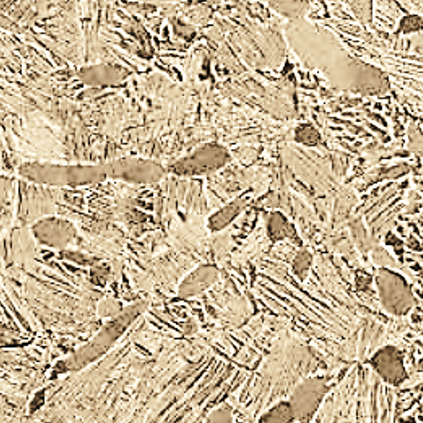
\includegraphics[width=0.8\linewidth]{pic/组织分析/910+510}
			%\caption{fig1}
		\end{minipage}%
	}%
	\subfigure[910℃固溶(水冷)550℃时效]{
		\begin{minipage}[t]{0.33\linewidth}
			\centering
			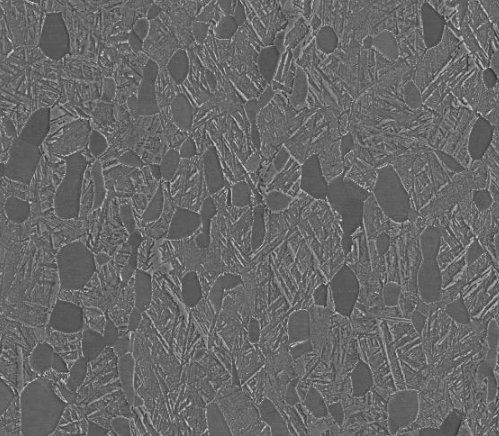
\includegraphics[width=0.8\linewidth]{pic/组织分析/910+550}
			%\caption{fig2}
		\end{minipage}%
	}%
	\subfigure[910℃固溶(油冷)590℃时效]{
		\begin{minipage}[t]{0.33\linewidth}
			\centering
			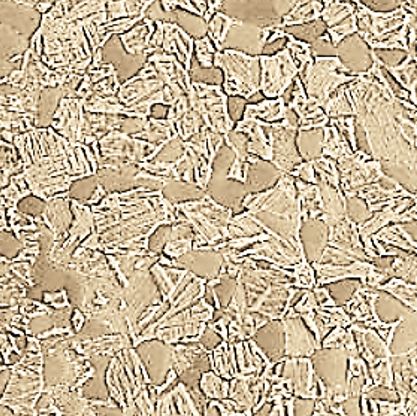
\includegraphics[width=0.8\linewidth]{pic/组织分析/910+590}
			%\caption{fig2}
		\end{minipage}
	}%
	\centering
	\caption{910℃固溶处理得到的组织}
	\label{fig:910c}
\end{figure}


随着温度的升高,当固溶温度到达$\alpha+\beta$相区附近时,如\ref{fig:950c}所示,最终的组织中会逐渐出现$\beta$相转变而成的针状$\alpha^\prime$相,与未完全转化的$\alpha$相交错分布。%这一结果也可以从XRD衍射图中看出来:所有组织中$\beta-Ti$的衍射峰几乎不存在,表明室温下不存在$\beta$相组织。
\begin{figure}[htbp]
	\centering
	\subfigure[950℃固溶(油冷)510℃时效]{
		\begin{minipage}[t]{0.33\linewidth}
			\centering
			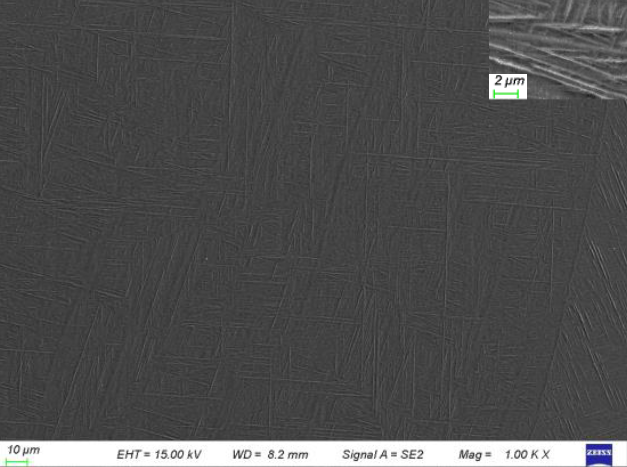
\includegraphics[width=0.8\linewidth]{pic/组织分析/950+510}
			%\caption{fig1}
		\end{minipage}%
	}%
	\subfigure[950℃固溶(水冷)550℃时效]{
		\begin{minipage}[t]{0.33\linewidth}
			\centering
			
\includegraphics[width=0.8\linewidth]{pic/组织分析/950+550}
			%\caption{fig2}
		\end{minipage}%
	}%
	\subfigure[950℃固溶(水冷)590℃时效]{
		\begin{minipage}[t]{0.33\linewidth}
			\centering
			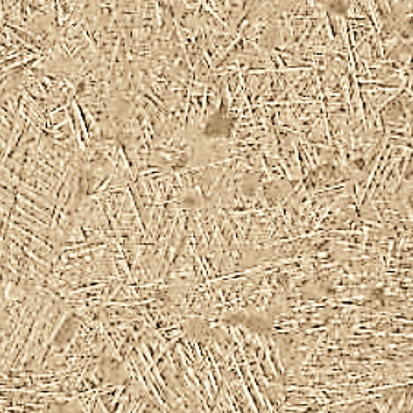
\includegraphics[width=0.8\linewidth]{pic/组织分析/950+590}
			%\caption{fig2}
		\end{minipage}
	}%
	\centering
	\caption{950℃固溶处理得到的组织}
	\label{fig:950c}
\end{figure}

当温度超过$\beta $转变终了线的时候,如\ref{fig:990c}所示,油冷、水冷得到的组织都是单一的针状$\alpha^\prime$,这表明组织中原本的$\alpha$相已经全部转变为$\alpha^\prime$相。

\begin{figure}[htbp]
	\centering
	\subfigure[990℃固溶(水冷)510℃时效]{
		\begin{minipage}[t]{0.33\linewidth}
			\centering
			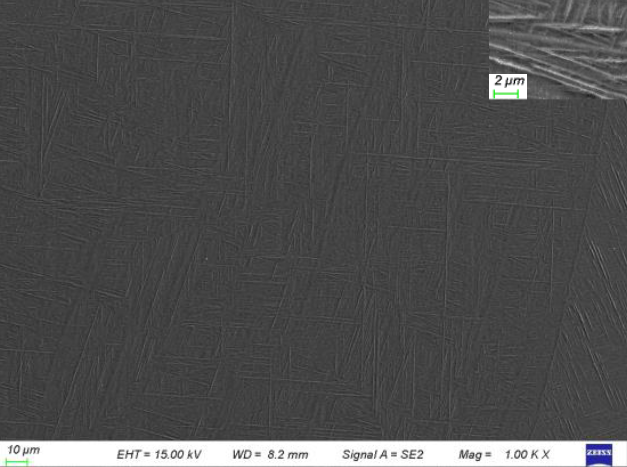
\includegraphics[width=0.8\linewidth]{pic/组织分析/990+510}
			%\caption{fig1}
		\end{minipage}%
	}%
	\subfigure[990℃固溶(油冷)550℃时效]{
		\begin{minipage}[t]{0.33\linewidth}
			\centering
			
\includegraphics[width=0.8\linewidth]{pic/组织分析/990+550}
			%\caption{fig2}
		\end{minipage}%
	}%
	\subfigure[990℃固溶(水冷)590℃时效]{
		\begin{minipage}[t]{0.33\linewidth}
			\centering
			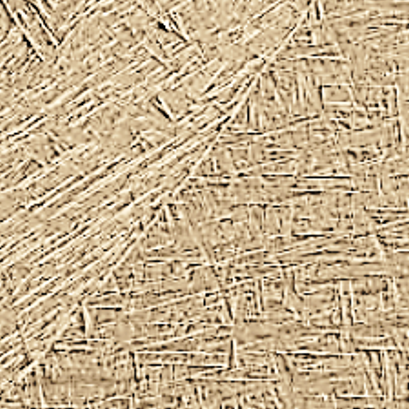
\includegraphics[width=0.8\linewidth]{pic/组织分析/990+590}
			%\caption{fig2}
		\end{minipage}
	}%
	\centering
	\caption{990℃固溶处理得到的组织}
	\label{fig:990c}
\end{figure}

力学分析结果如\ref{fig:Gqy}所示,图中的几组数据都是经过了水冷处理,并根据时效温度的不同分为成了三组(依次为510℃、550℃、590℃),从图后两组的对比中可以看出,固溶温度在950℃附近的合金在处理后,抗拉强度比910℃、990℃都高;而当固溶温度达到990℃的时候,从第一、三组可以看到延伸率显著下降,这是因为固溶温度过高,组织中生成了魏氏组织的缘故。


\begin{figure}[h!]
	\centering
	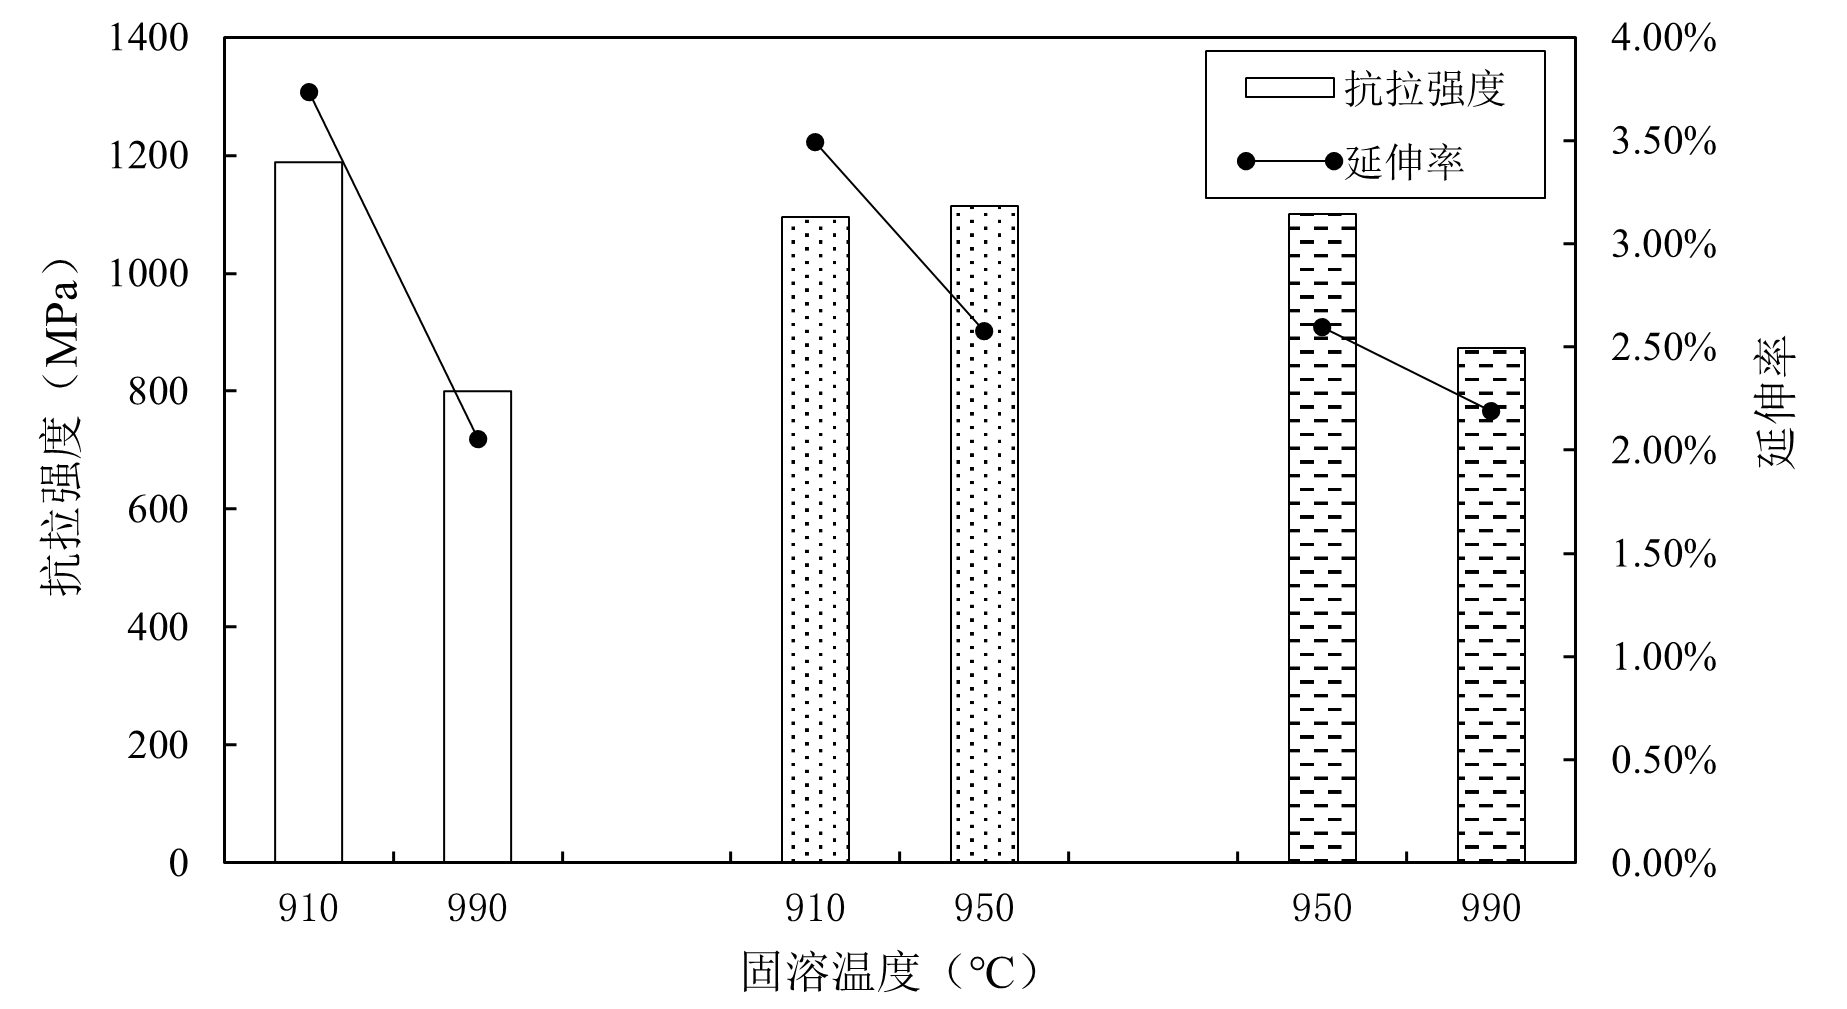
\includegraphics[width=1\linewidth]{pic/固溶温度与屈服强度、延伸率的关系}
	\caption{固溶温度与屈服强度、延伸率的关系}
	\label{fig:Gqy}
\end{figure}

\section{冷却速度对组织性能的影响}
本设计采用了两种淬火方式:油冷与水冷。由于淬火油的热传导速度相对较低,淬火时冷却速度较慢,与水冷相比,组织处于高温时的时间更久,最后形成了不同的组织形貌。下面就强度较高的950℃组来进行分析。
合金在加热过程中,随着温度的升高,$\alpha$相逐渐发生相变转变成$\beta$相,温度越高,转变的量越多。由于油冷情况下的冷却速度比水冷的小,组织中的初生$\alpha $相的生长时间更久,形成的等轴$\alpha $相尺寸较大,$\beta $相中合金元素可以发生扩散,发生扩散型相变,最终形成与珠光体类似的$\alpha $片层与$\beta $片层相间分布的$\beta $转变组织,亦即双态组织;而水冷的速度比较快,本设计所用小试样的比表面积相对较大,导致冷却极快,导致$\beta \to\alpha $的扩散型相变来不及发生,$\beta $相只能通过类似马氏体相变的非扩散型晶格切变来进行相变,生成了$\alpha^{\prime}$马氏体,水冷后最终组织中含有$\alpha $相与$\alpha^{\prime} $相。
%由于本实验采取的是正交实验方法来探究不同因素的影响,其中冷却方式设置了两种,不能根据控制变量法来进行绝对准确地分析,这里根据关联性来进行分析,由于 $F_{1冷}=1.919 > F_{1时}=0.177$,可见时效温度对于力学性能的相关性较小。

罗文忠等表明:时效处理过程中,初生$\alpha$相的含量与分布对合金最终的力学性能影响较大,尤其是当初生$\alpha$相的含量在$15\% \sim 20\%$时,随着其含量的增加,组织的塑性逐渐增加。不论是如\ref{910}的910℃固溶处理,还是经过如\ref{950}温度更高的950℃处理后,油冷得到的合金延伸率都比较高,可见油冷后得到的组织$\alpha$相含量更多,具有更好的塑性。
\begin{figure}[h!]
	\centering
			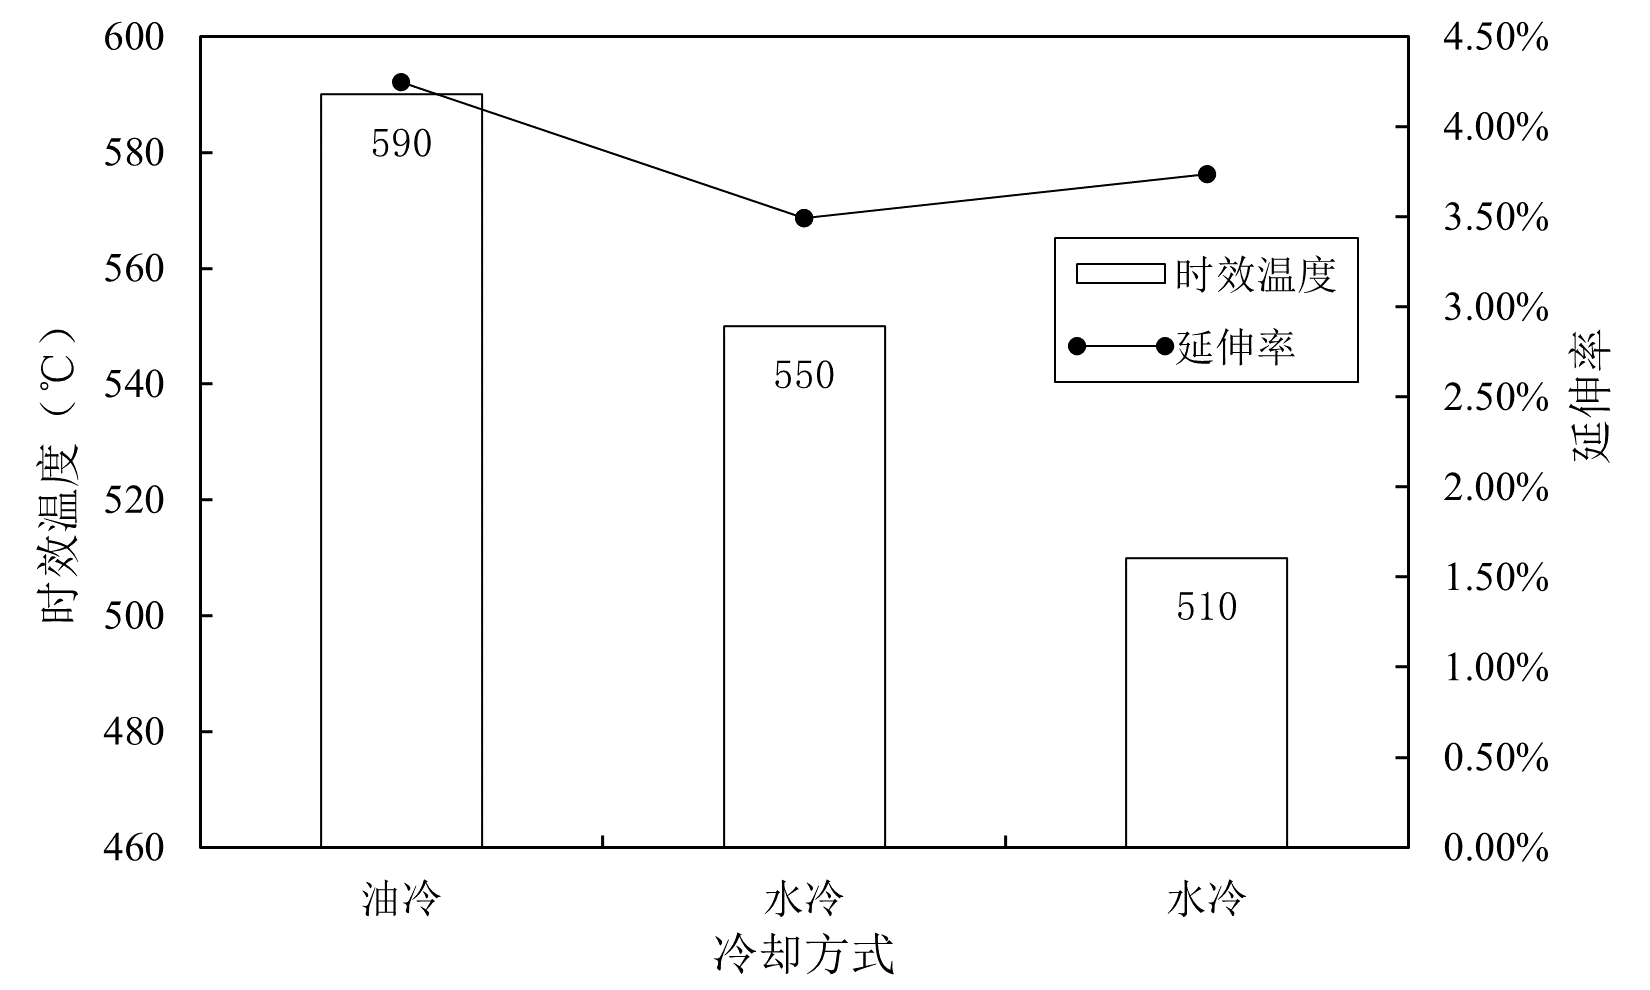
\includegraphics[width=1\linewidth]{pic/910℃固溶处理后不同冷却方式下组织的力学性能特点}
	\caption{910℃固溶处理后不同冷却方式下组织的力学性能特点}
	\label{910}
\end{figure}
\begin{figure}[h!]
	\centering
	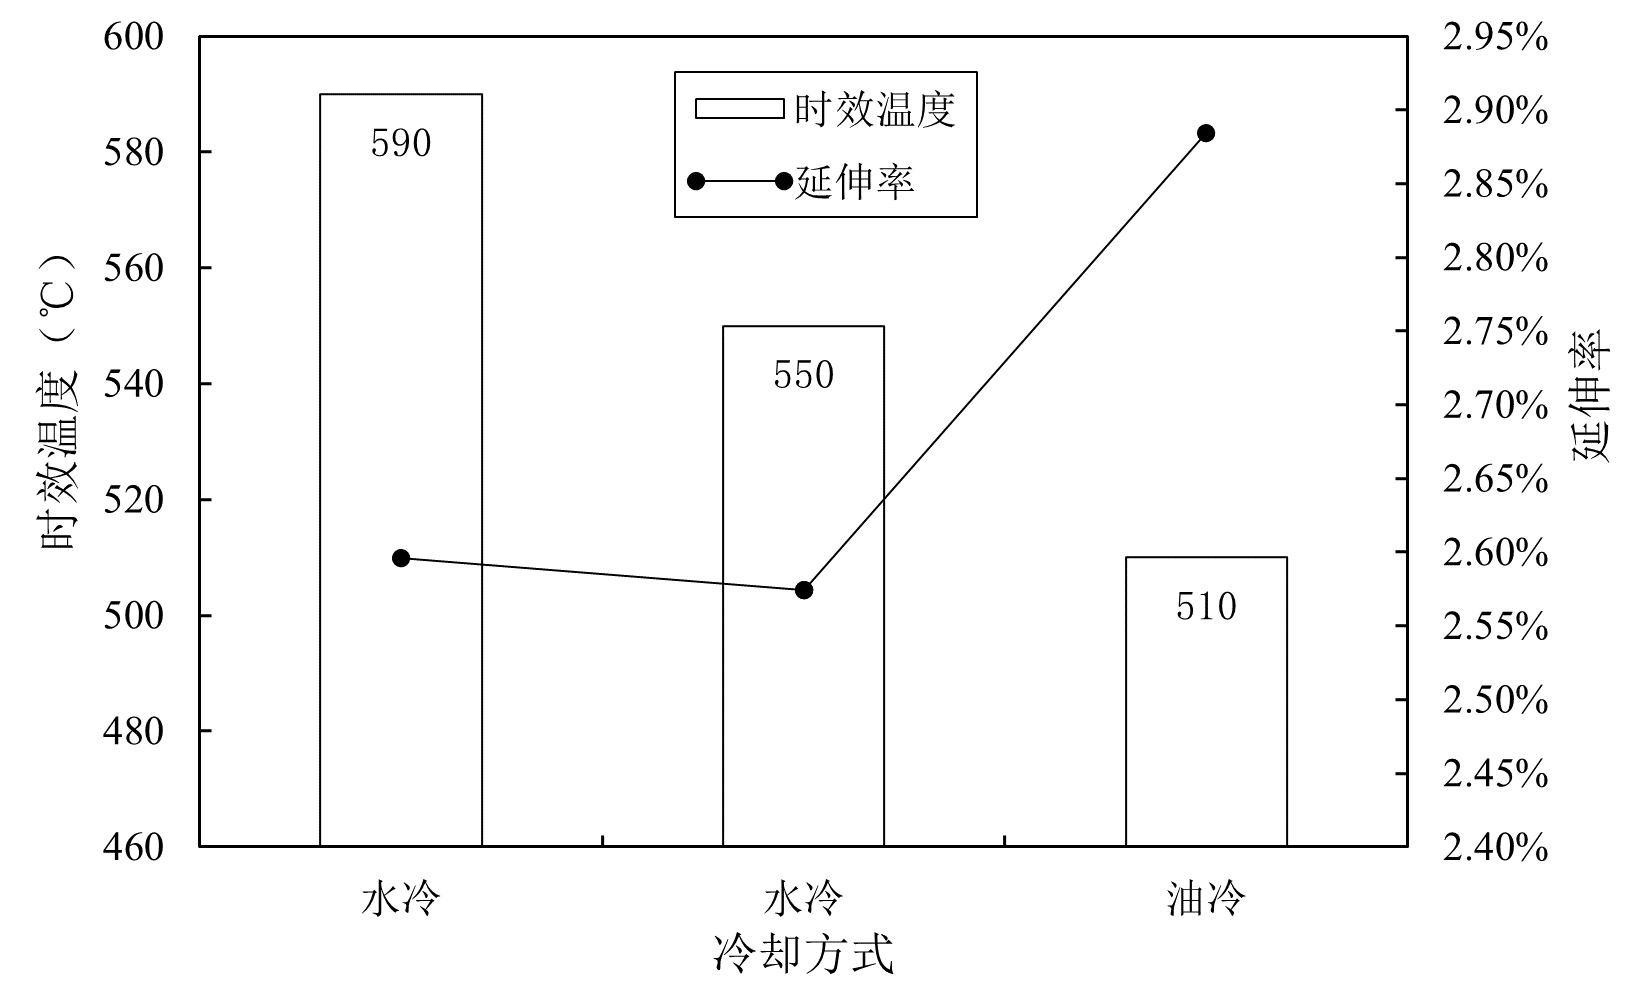
\includegraphics[width=1\linewidth]{pic/950℃固溶处理后不同冷却方式下组织的力学性能特点}
	\caption{950℃固溶处理后不同冷却方式下组织的力学性能特点}
	\label{950}
\end{figure}

\section{时效温度对组织性能的影响}
时效温度在热处理过程中主要是影响了亚稳$\beta $相的分解。

从\ref{fig:sqy}可以看出,不同时效温度下合金的抗拉强度与延伸率的差异并不大,可见在510℃$\sim$ 590℃之间进行时效时,对于合金的的力学性能影响较小,这同正交实验分析的结果是一致的。

经过910℃固溶10min后水冷的合金在500℃到600℃内时效60min后,强度得到了明显提升,但塑性有所下降。而且时效温度越高,抗拉强度越低,延伸率则先减小后增大,其中抗拉强度在510℃固溶时达到最大,为1138MPa,延伸最大600℃时的$ 3.73\% $,与对照组相比,强度上升了17.81$ \% $,延伸率下降了$ 45.33\% $。
\begin{figure}[h!]
	\centering
	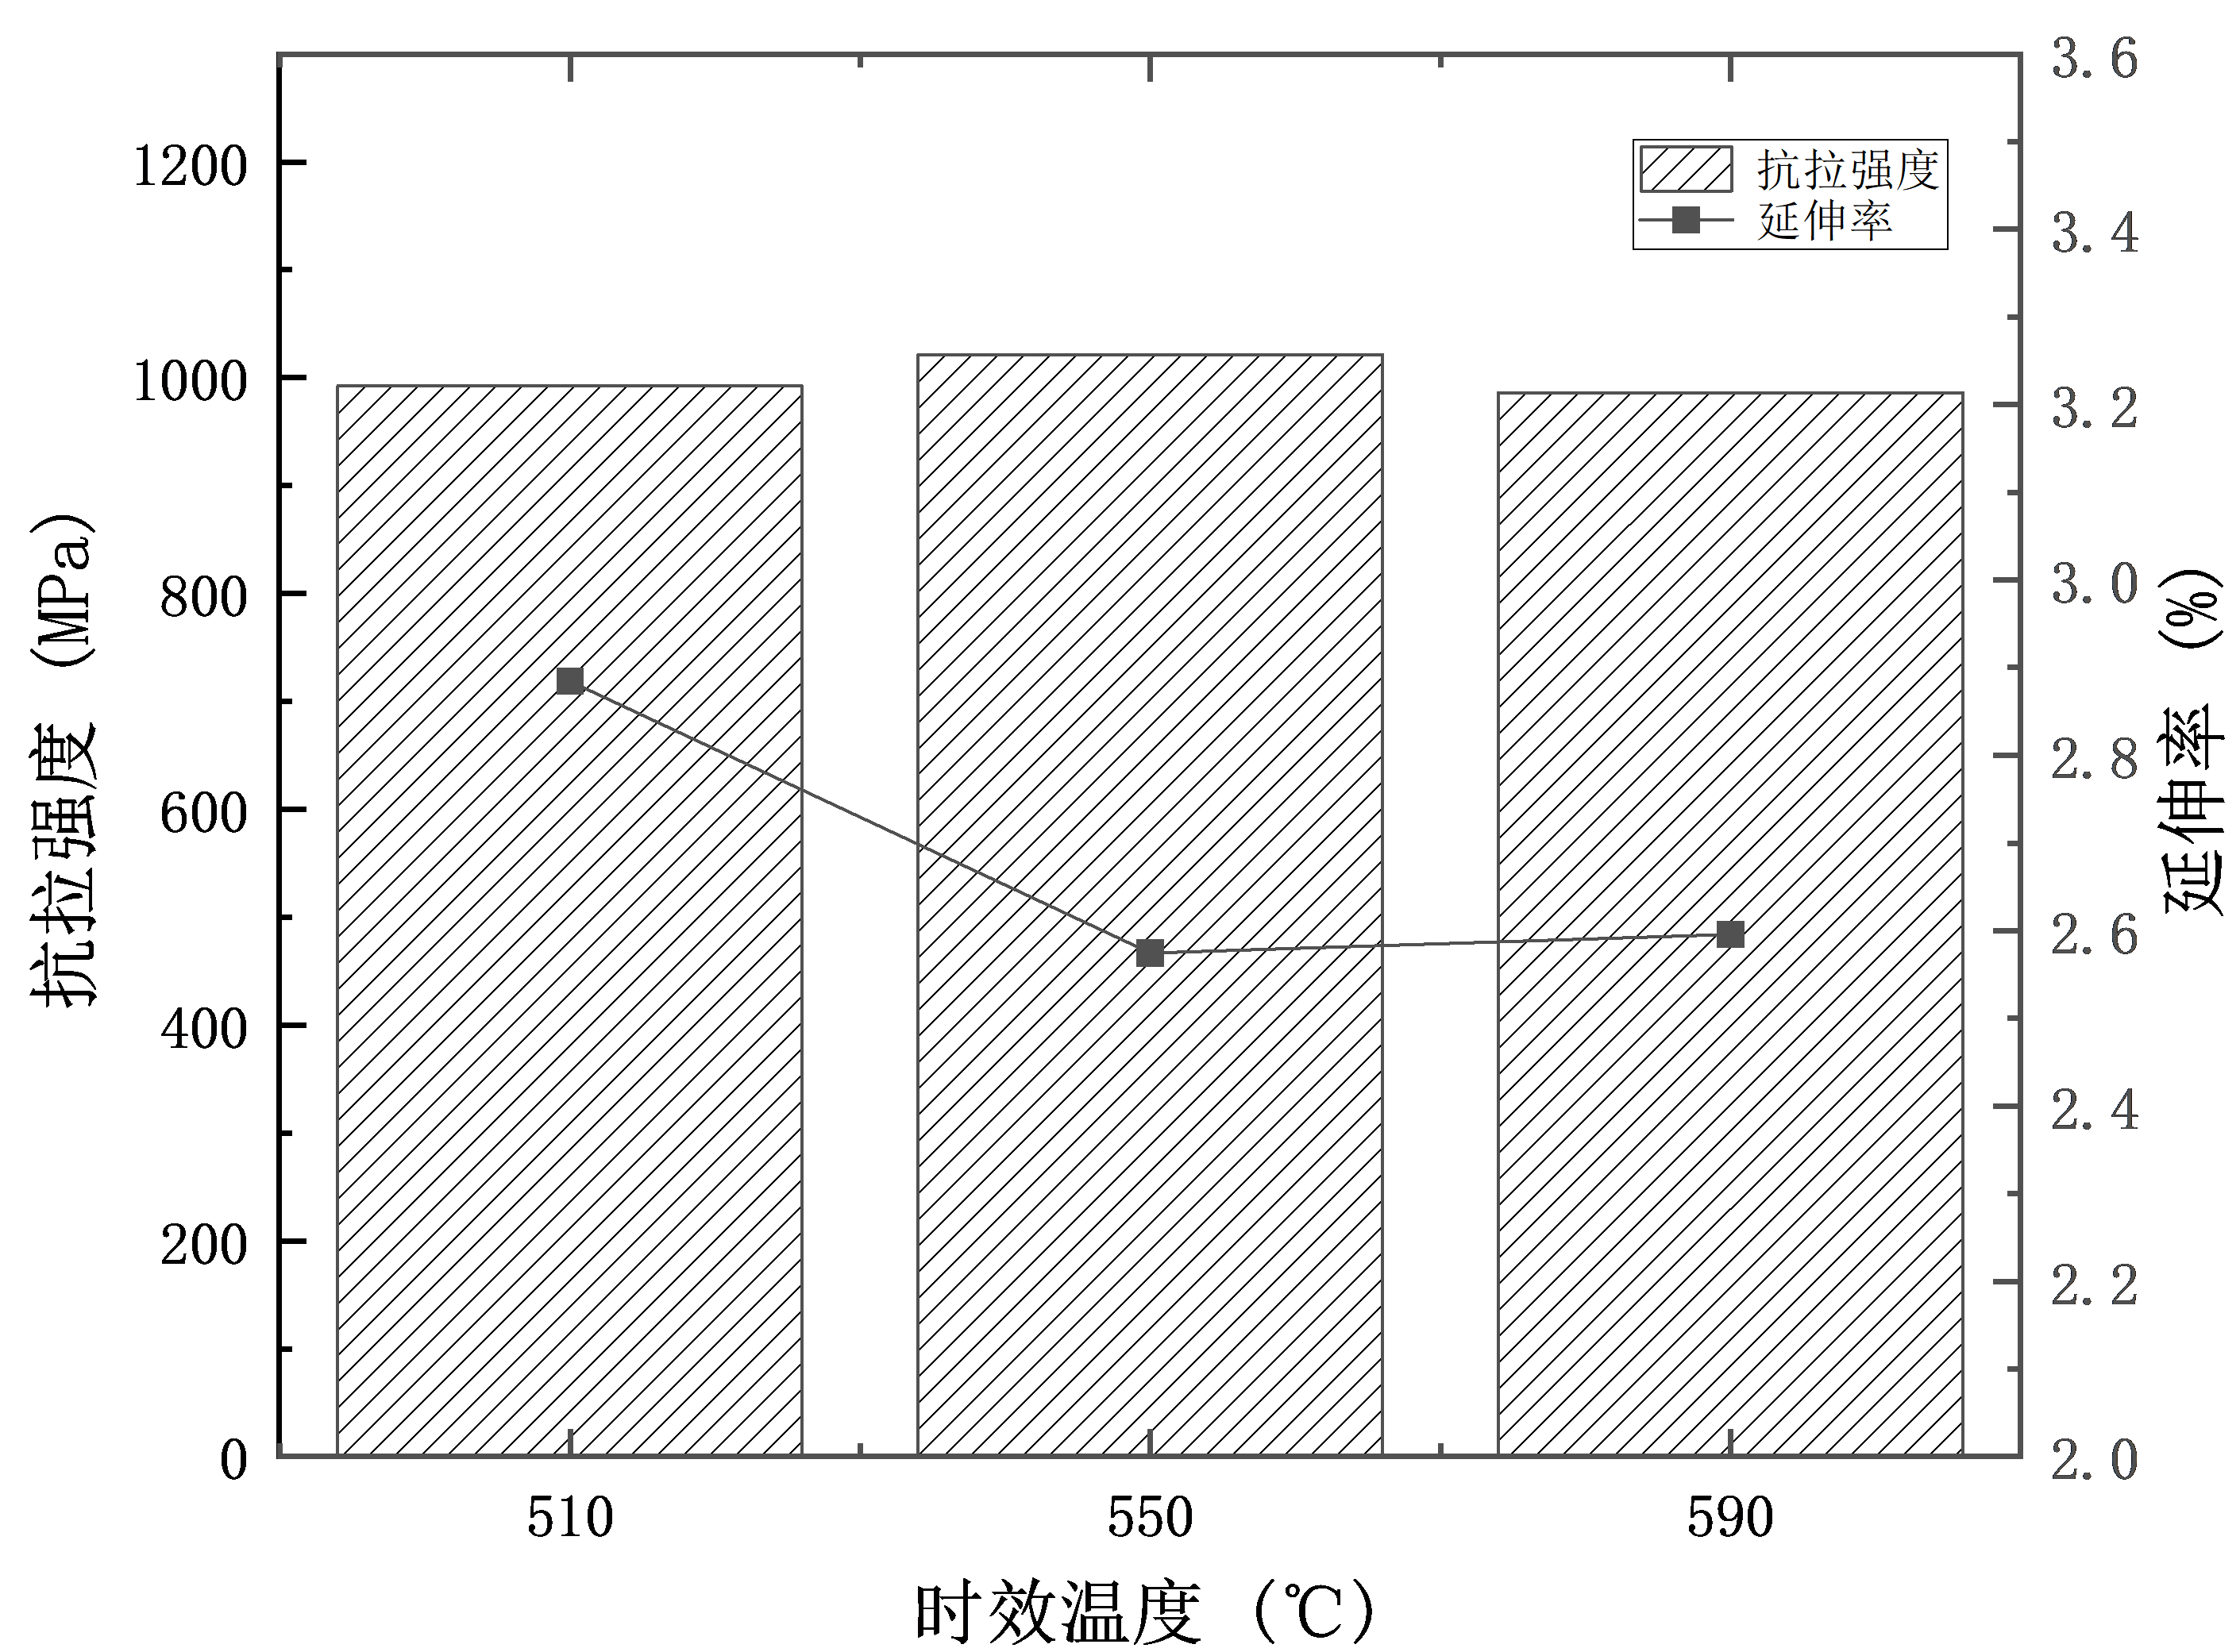
\includegraphics[width=0.7\linewidth]{pic/时效温度与屈服强度、延伸率的关系}
	\caption{时效温度与屈服强度、延伸率的关系}
	\label{fig:sqy}
\end{figure}


%
%\section{相变点以下固溶处理对组织性能的影响}
%			\begin{figure}[htbp]
%				\centering
%				\subfigure[910℃固溶(油冷)+590℃时效]{
%					\begin{minipage}[t]{0.33\linewidth}
%						\centering
%						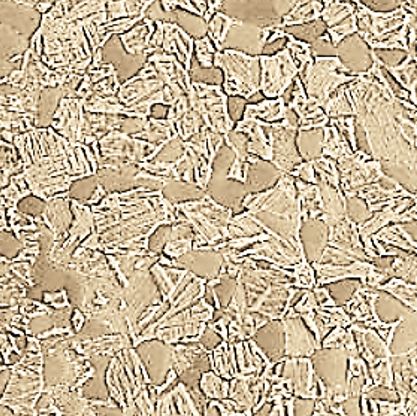
\includegraphics[width=0.9\linewidth]{pic/组织分析/910+590}
%						\label{fig:910590}
%					\end{minipage}%
%				}%
%				\subfigure[910℃固溶(水冷)+550℃时效]{
%				\begin{minipage}[t]{0.33\linewidth}
%					\centering
%					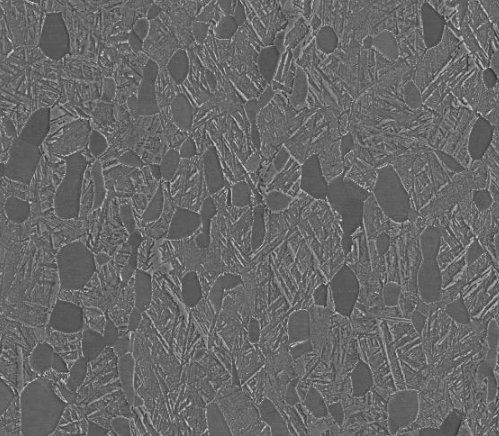
\includegraphics[width=0.9\linewidth]{pic/组织分析/910+550}
%					\label{fig:910550}
%					%\caption{fig2}
%				\end{minipage}%
%			}%
%				\subfigure[910℃固溶(水冷)+510℃时效]{
%					\begin{minipage}[t]{0.33\linewidth}
%						\centering
%						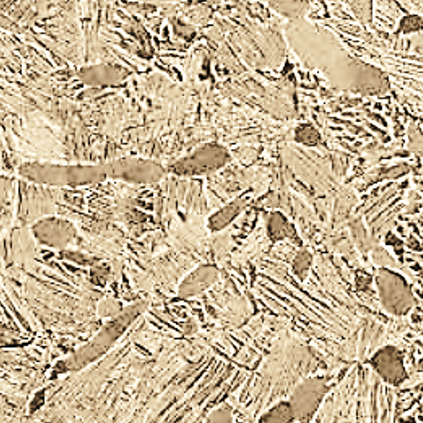
\includegraphics[width=0.9\linewidth]{pic/组织分析/910+510}
%						\label{fig:910510}
%						%\caption{fig2}
%					\end{minipage}%
%				}%
%				\centering
%				\label{910}
%				\caption{不同冷却方式下的 TC4 钛合金显微组织}
%			\end{figure}
%			\begin{figure}[h!]
%			\centering
%			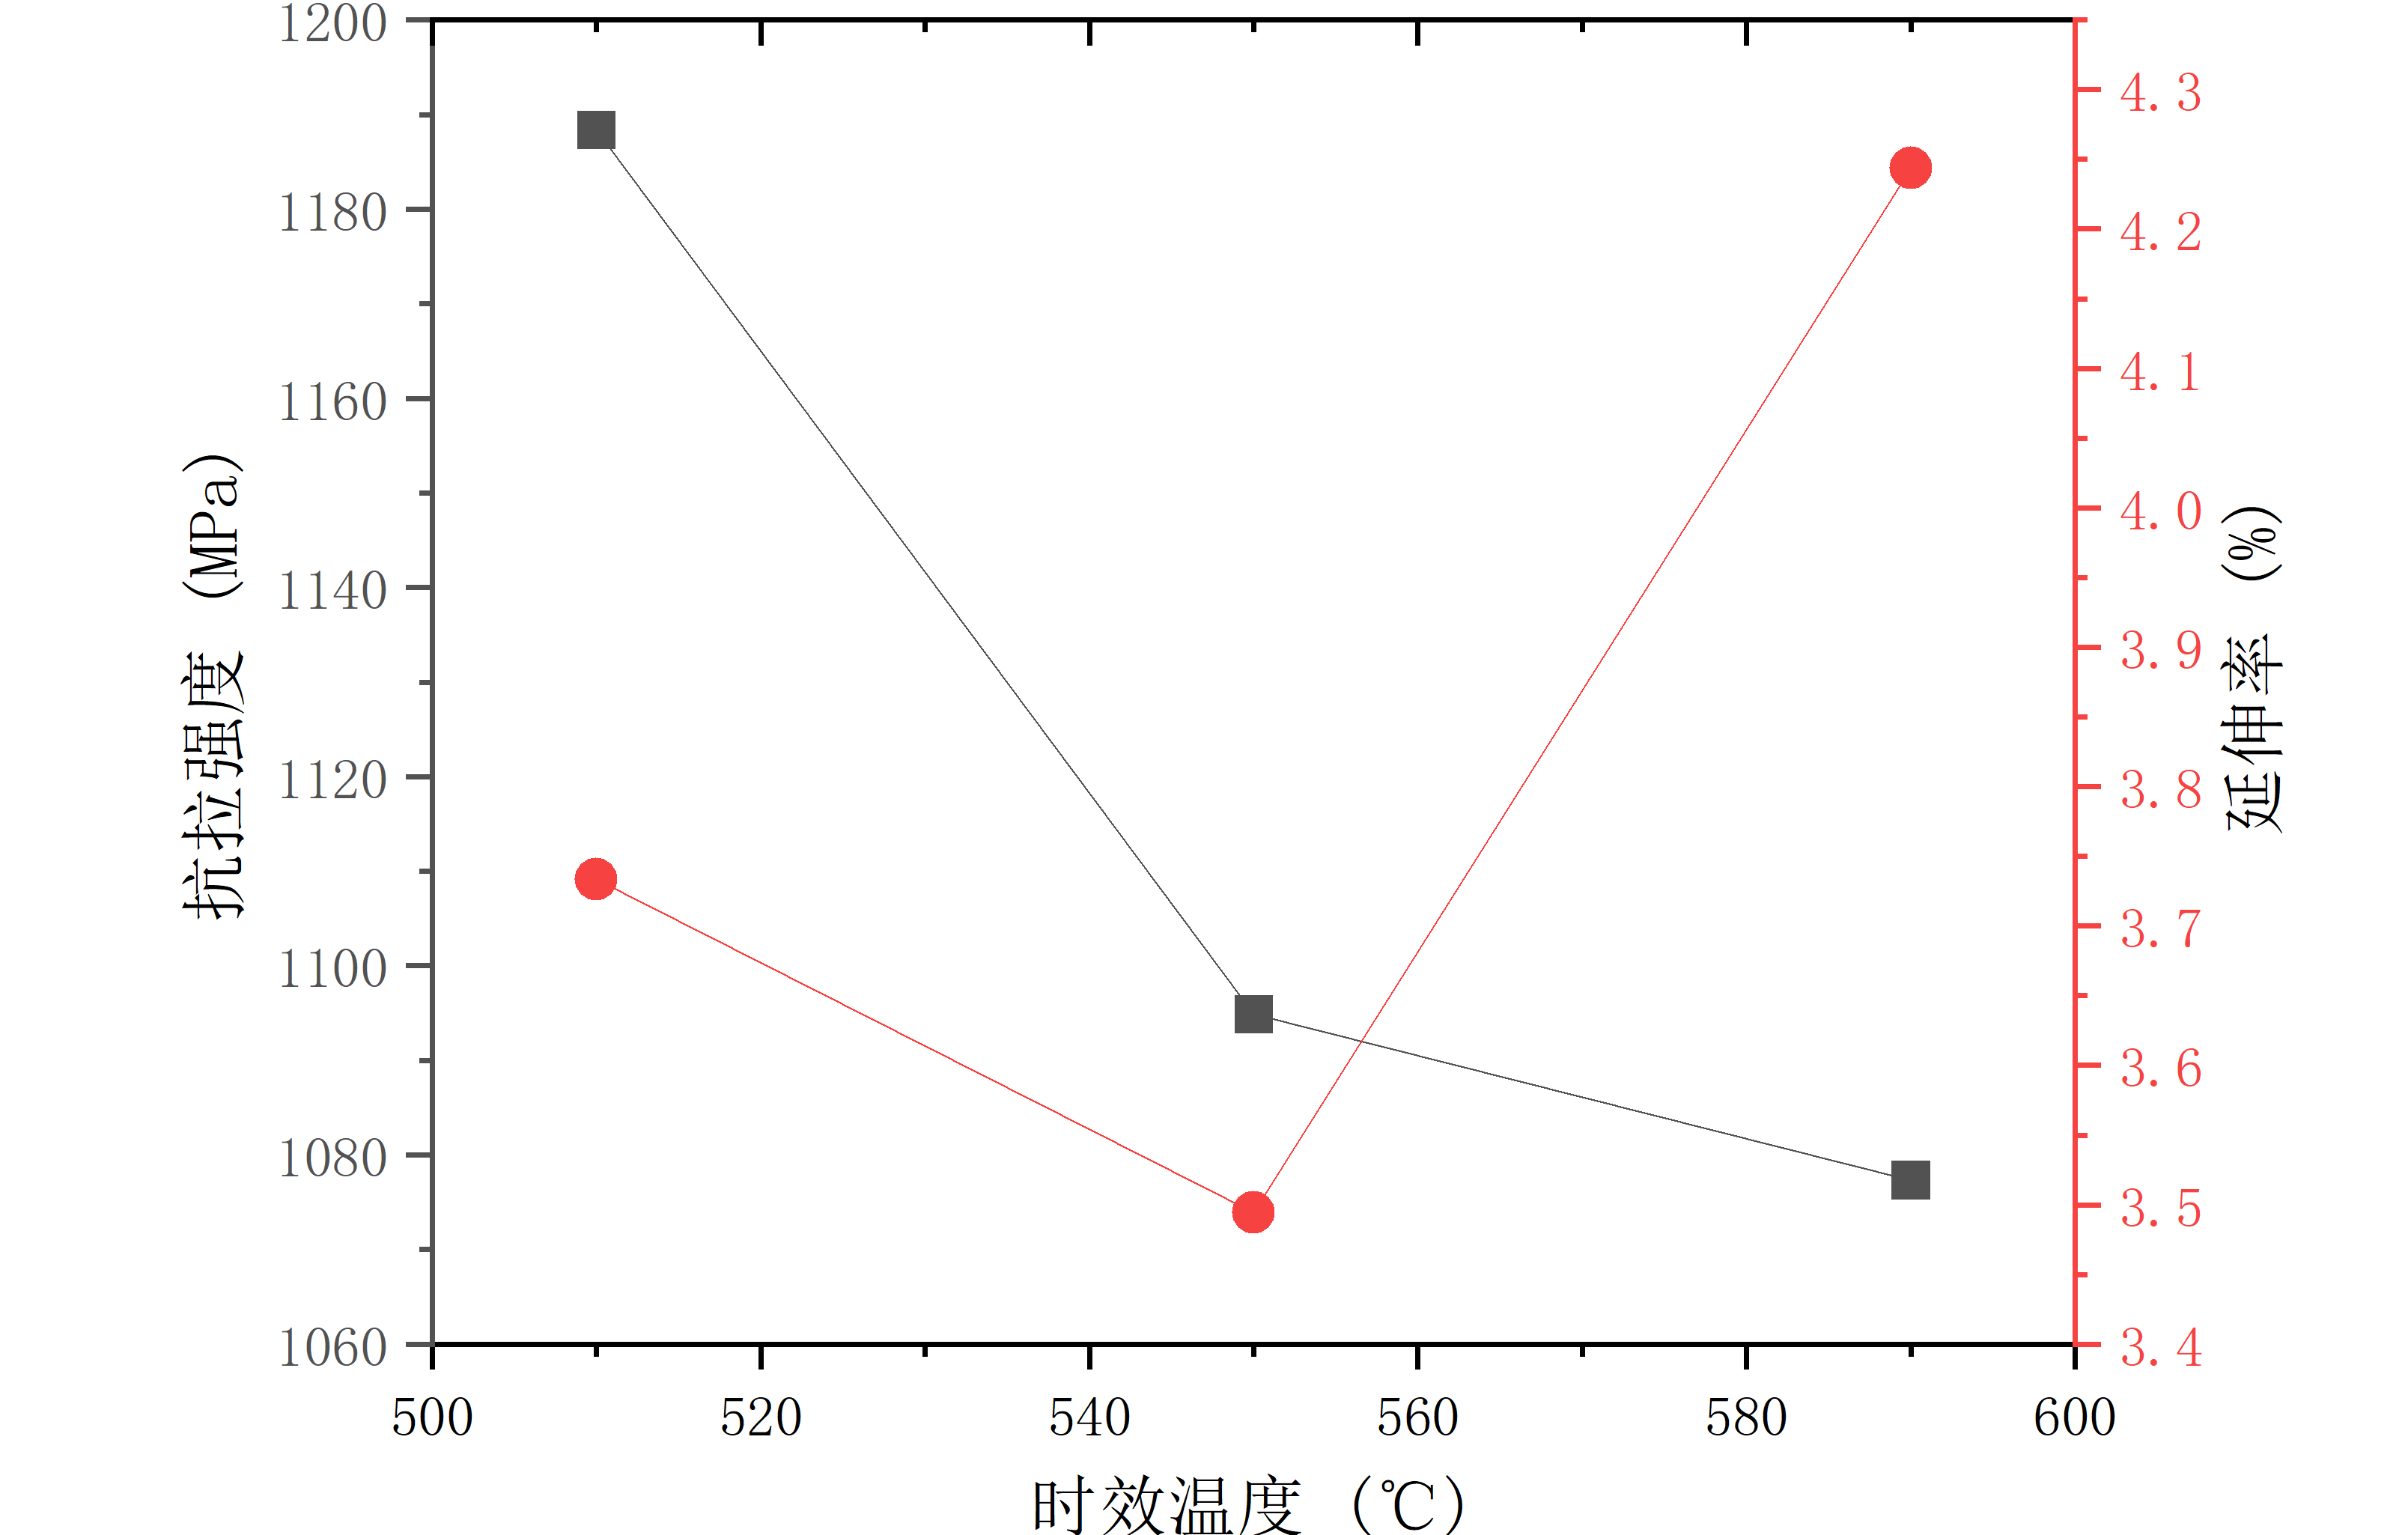
\includegraphics[width=0.7\linewidth]{pic/910分析}
%			\label{fig:910}
%			\caption{910℃固溶组的时效温度与抗拉强度、延伸率的关系}
%
%		\end{figure}
%			前三组试样的固溶温度为910℃,低于所用的TC4合金的相变点973℃,处于在相变点以下,时效温度都在$ 500\sim 600$℃之间。组织形貌如\ref{910}所示。
%
%			\textbf{  组织分析:}在处理过程中,随着温度的升高,$ \alpha $相逐渐向$ \beta $相转变,在达到设定的温度时,组织由初生等轴$ \alpha $相和$ \beta $相组成。经过水或淬火油的快速冷却后,组织发生马氏体转变,由图\ref{fig:910510}可见,冷却后的组织有等轴初生$ \alpha $相和针状马氏体组成。
%
%			\textbf{  性能分析:}该组试样的一个典型特点是固溶后的初生等轴$\alpha $相含量较多,钛合金经过热处理后的塑性与合金的微观组织分布关系密切,组织中尤其是初生等轴$\alpha $相的含量对塑性的影响最大\cite{zouhaibeiTC4taihejinrechuliqianghuagongyijixiangbianhangweiyanjiu2019},当初生等轴$\alpha $相的含量为$ 15\%\~20\% $之间时,随着等轴$\alpha $相的增加,材料的塑性逐渐增加,从图可以看出,该组材料的延伸率基本上达到了$ 3\% $以上,塑性较好。
%
%			\textbf{  固溶冷速:}由于油冷情况下的冷却速度比水冷的小,组织中的初生$\alpha $相的生长时间更久,形成的等轴$\alpha $相尺寸较大,$\beta $相中合金元素可以发生扩散,发生扩散型相变,最终形成与珠光体类似的$\alpha $片层与$\beta $片层相间分布的$\beta $转变组织,亦即双态组织;而水冷的速度比较快,本设计所用小试样的比表面积相对较大,导致冷却极快,导致$\beta \to\alpha $的扩散型相变来不及发生,$\beta $相只能通过类似马氏体相变的非扩散型晶格切变来进行相变,生成了$\alpha^{\prime}$马氏体,水冷后最终组织中含有$\alpha $相与$\alpha^{\prime} $相。
%
%			\textbf{  时效温度:}由\ref{fig:910}可得,经过910℃固溶10min后水冷的合金在500℃到600℃内时效60min后,强度得到了明显提升,但塑性有所下降。而且时效温度越高,抗拉强度越低,延伸率则先减小后增大,其中抗拉强度在510℃固溶时达到最大,为1138MPa,延伸最大600℃时的$ 3.73\% $,与对照组相比,强度上升了17.81$ \% $,延伸率下降了$ 45.33\% $。
%			\newpage
%\section{两相区固溶处理对组织性能的影响}
%
%\begin{figure}[htbp]
%	\centering
%	\subfigure[950℃固溶(油冷)+550℃时效]{
%		\begin{minipage}[t]{0.33\linewidth}
%			\centering
%			
\includegraphics[width=0.9\linewidth]{pic/组织分析/950+550}
%			\label{fig:950550}
%		\end{minipage}%
%	}%
%	\subfigure[950℃固溶(水冷)+590℃时效]{
%		\begin{minipage}[t]{0.33\linewidth}
%			\centering
%			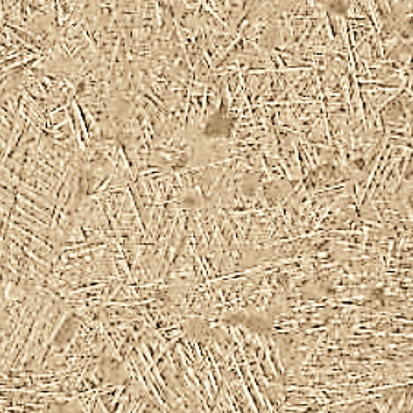
\includegraphics[width=0.9\linewidth]{pic/组织分析/950+590}
%			\label{fig:950590}
%			%\caption{fig2}
%		\end{minipage}%
%	}%
%	\subfigure[950℃固溶(水冷)+510℃时效]{
%		\begin{minipage}[t]{0.33\linewidth}
%			\centering
%			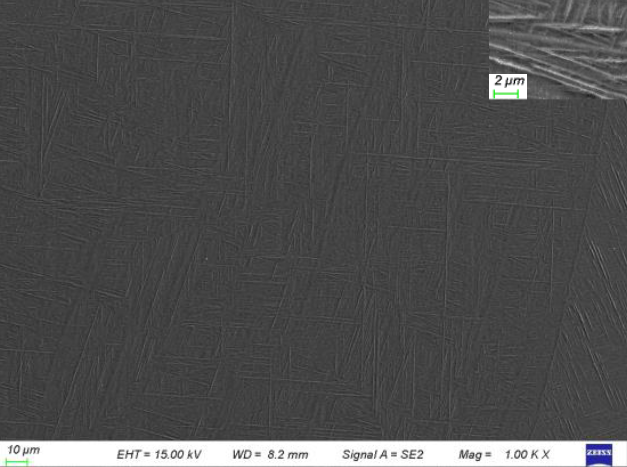
\includegraphics[width=0.9\linewidth]{pic/组织分析/950+510}
%			\label{fig:950510}
%			%\caption{fig2}
%		\end{minipage}%
%	}%
%	\centering
%	\label{950}
%	\caption{双相区固溶的 TC4 钛合金显微组织}
%\end{figure}
%
%		\begin{figure}[h!]
%			\centering
%			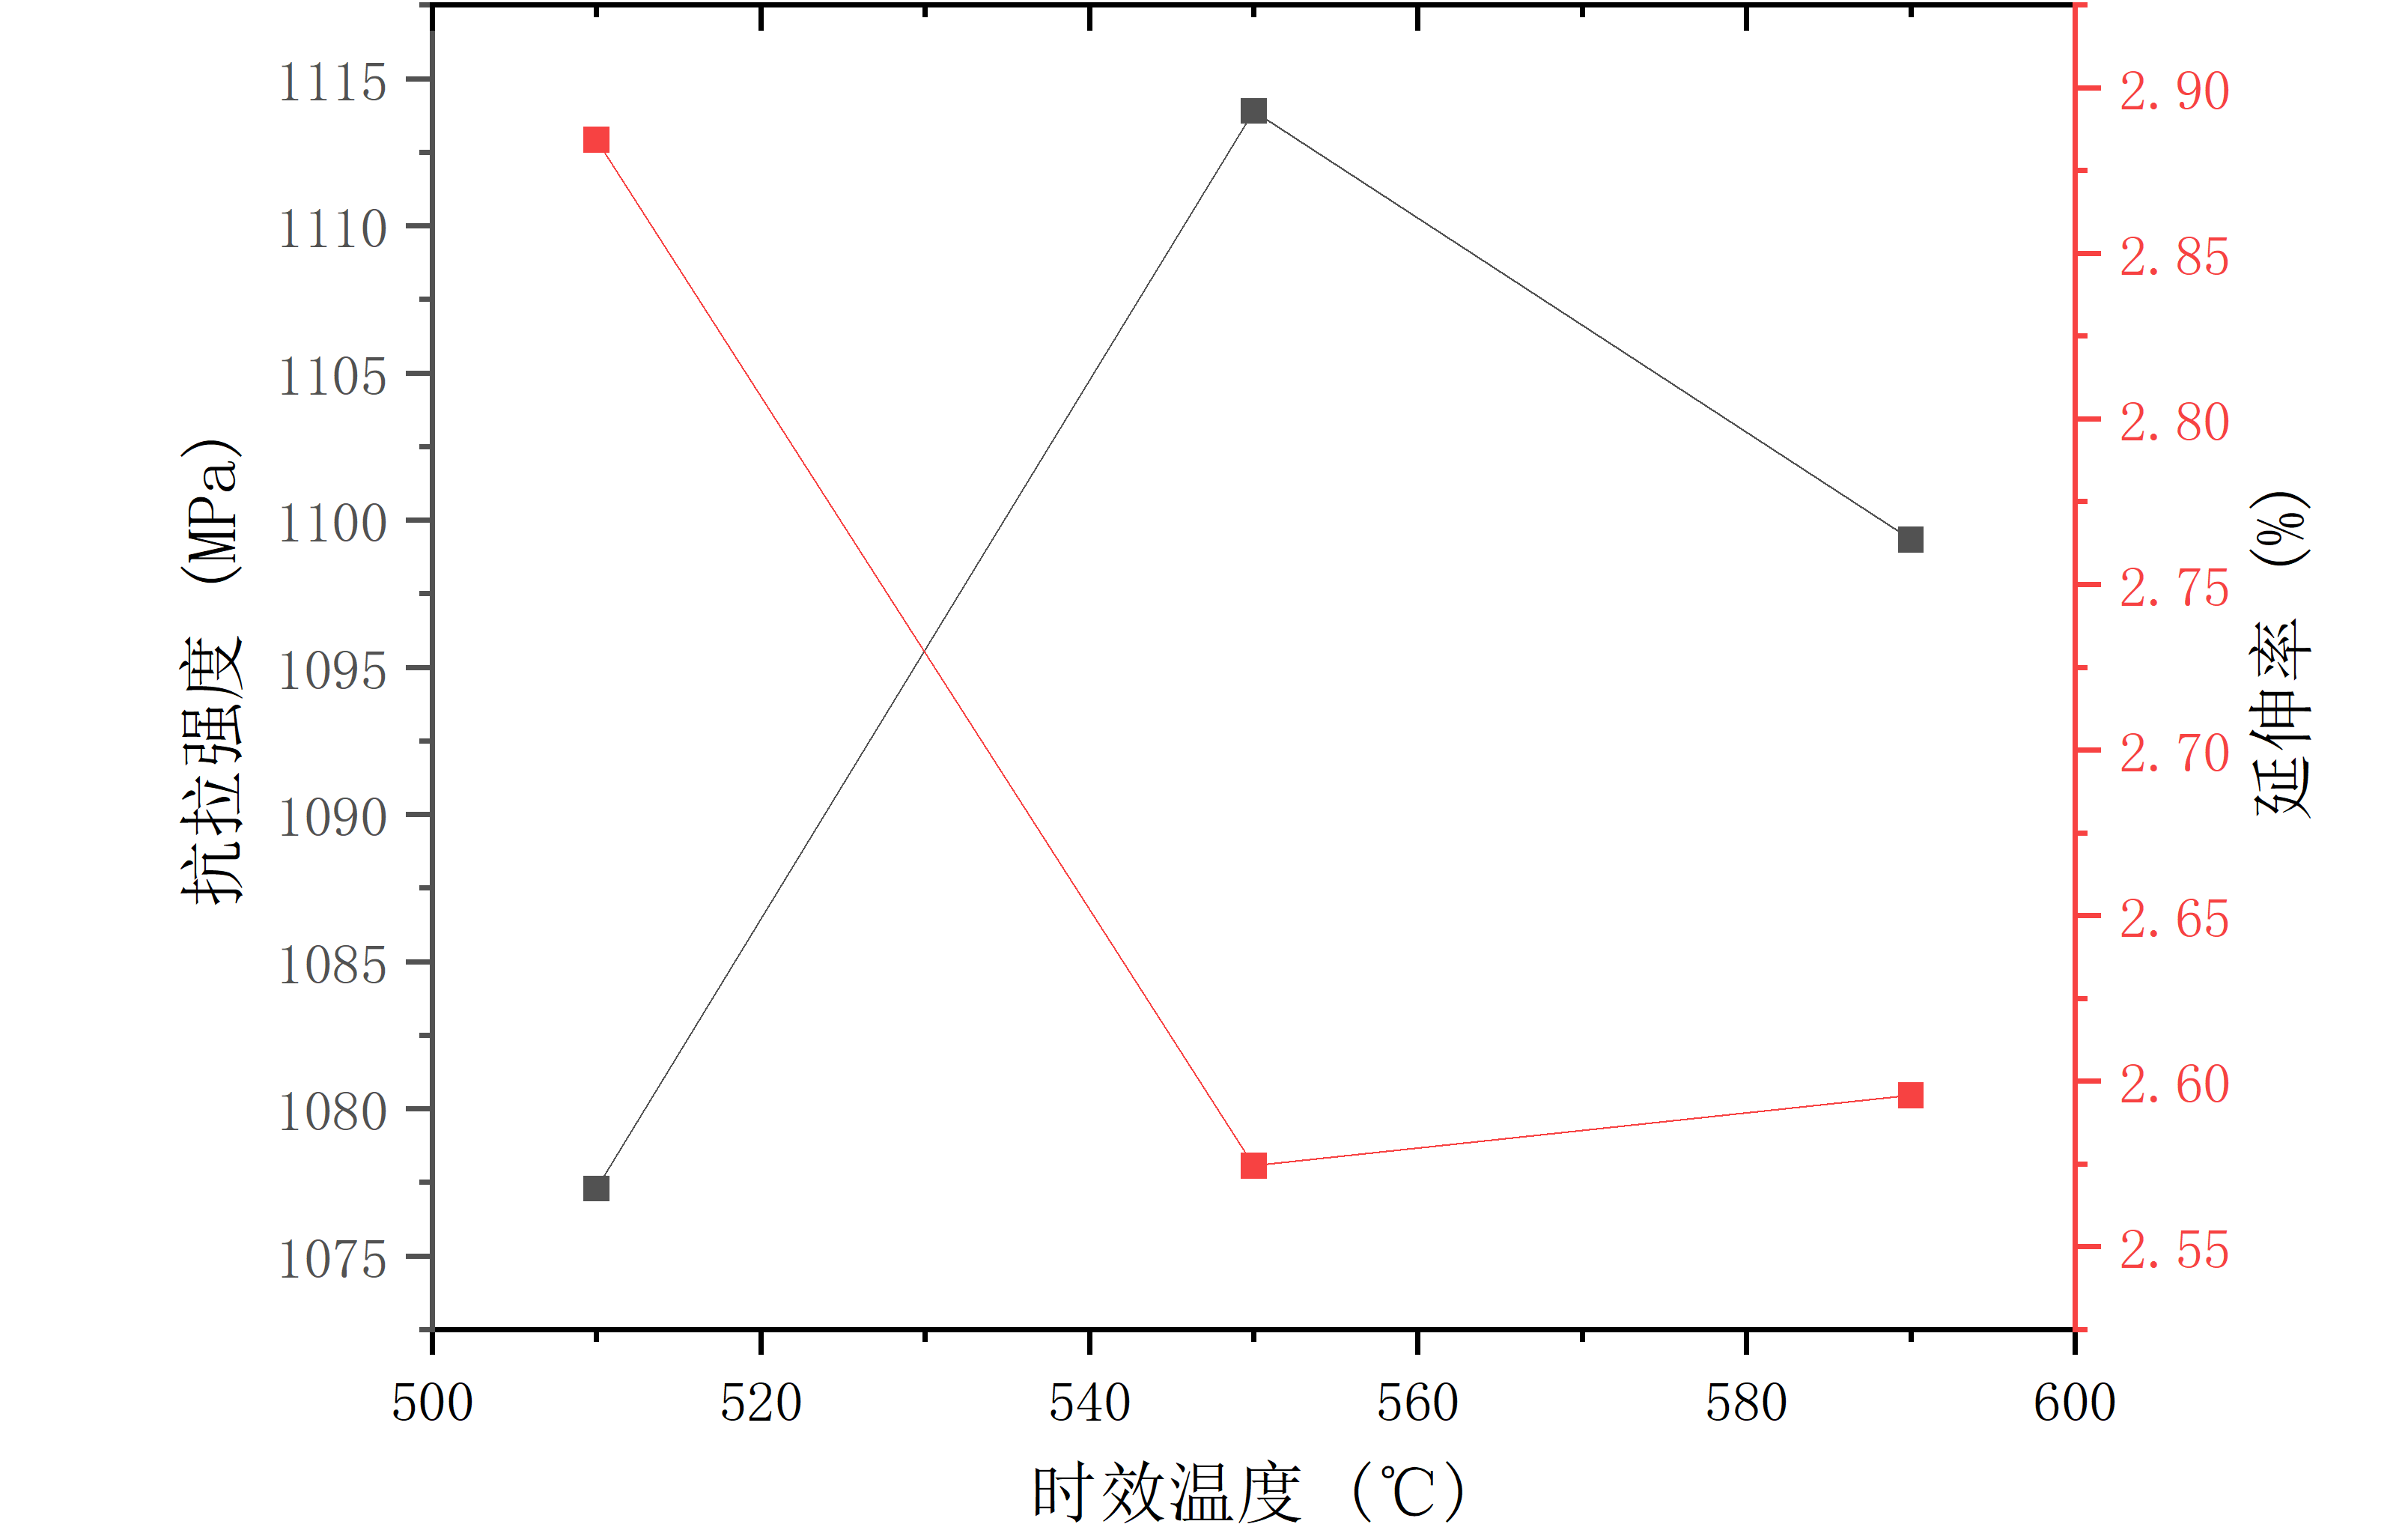
\includegraphics[width=0.7\linewidth]{pic/950分析}
%			\caption{950分析}
%			\label{fig:950}
%		\end{figure}
%
%\textbf{  组织分析:}如\ref{fig:950590}所示:在$ \alpha+\beta $两相区进行固溶后水冷,得到初生等轴$ \alpha $相与细针状$ \alpha^{\prime}$马氏体交错组成的双态组织,与第一大组相比,由于加热温度偏高,$ \beta $相长大,形成的$ \beta $相比较粗大。
%
%\textbf{  性能分析:}从\ref{950}可以看出,这三组的抗拉均强度明显高于对照组,说明经过固溶和时效处理后,钛合金的综合力学性能得到了提升。然而延伸率却明显降低,说明处理后材料的塑性变差。
%
%\textbf{  固溶冷速:}水冷的冷却速度比油冷快,导致材料的强化相数量增多,也会导致较大的晶粒尺寸。而油冷则相反,会产生更细小的强化相和晶粒。
%
%\textbf{  时效温度:}由\ref{fig:950}可得,时效温度越高,亚稳定$ \beta $相的分解越充分,可以得到较好的强度与塑韧性,但当时效温度过高时,组织变粗大,性能较差。
%
%\section{相变点以上固溶处理对组织性能的影响}
%如\ref{fig:990590}所示:在$ \alpha+\beta $两相区进行固溶后冷却,得到粗大的原始$ \beta $相晶粒内部分布着单一的细针状马氏体,
%\begin{figure}[htbp]
%	\centering
%	\subfigure[990℃固溶(水冷)+550℃时效]{
%		\begin{minipage}[t]{0.33\linewidth}
%			\centering
%			
\includegraphics[width=0.9\linewidth]{pic/组织分析/990+550}
%			\label{fig:990550}
%		\end{minipage}%
%	}%
%	\subfigure[990℃固溶(水冷)+590℃时效]{
%		\begin{minipage}[t]{0.33\linewidth}
%			\centering
%			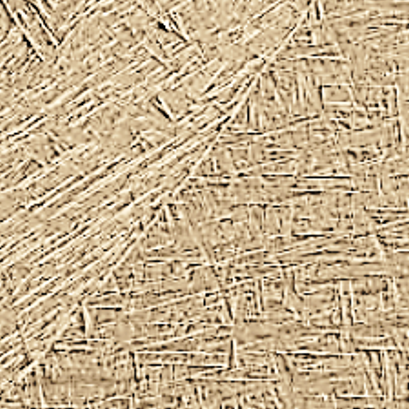
\includegraphics[width=0.9\linewidth]{pic/组织分析/990+590}
%			\label{fig:990590}
%			%\caption{fig2}
%		\end{minipage}%
%	}%
%	\subfigure[990℃固溶(油冷)+510℃时效]{
%		\begin{minipage}[t]{0.33\linewidth}
%			\centering
%			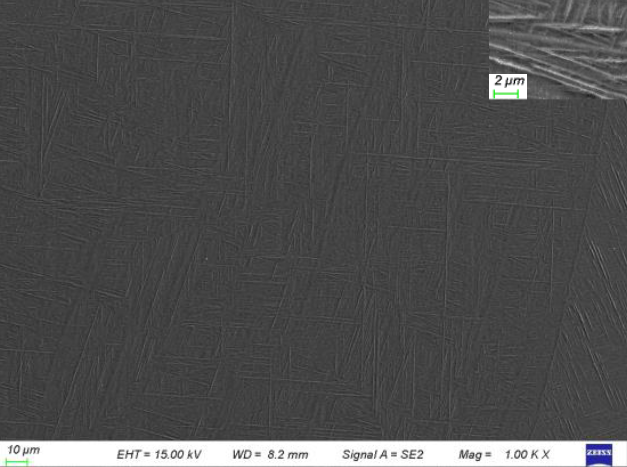
\includegraphics[width=0.9\linewidth]{pic/组织分析/990+510}
%			\label{fig:990510}
%			%\caption{fig2}
%		\end{minipage}%
%	}%
%	\centering
%	\caption{双相区固溶的 TC4 钛合金显微组织}
%\end{figure}
%
%\begin{figure}[h!]
%	\centering
%	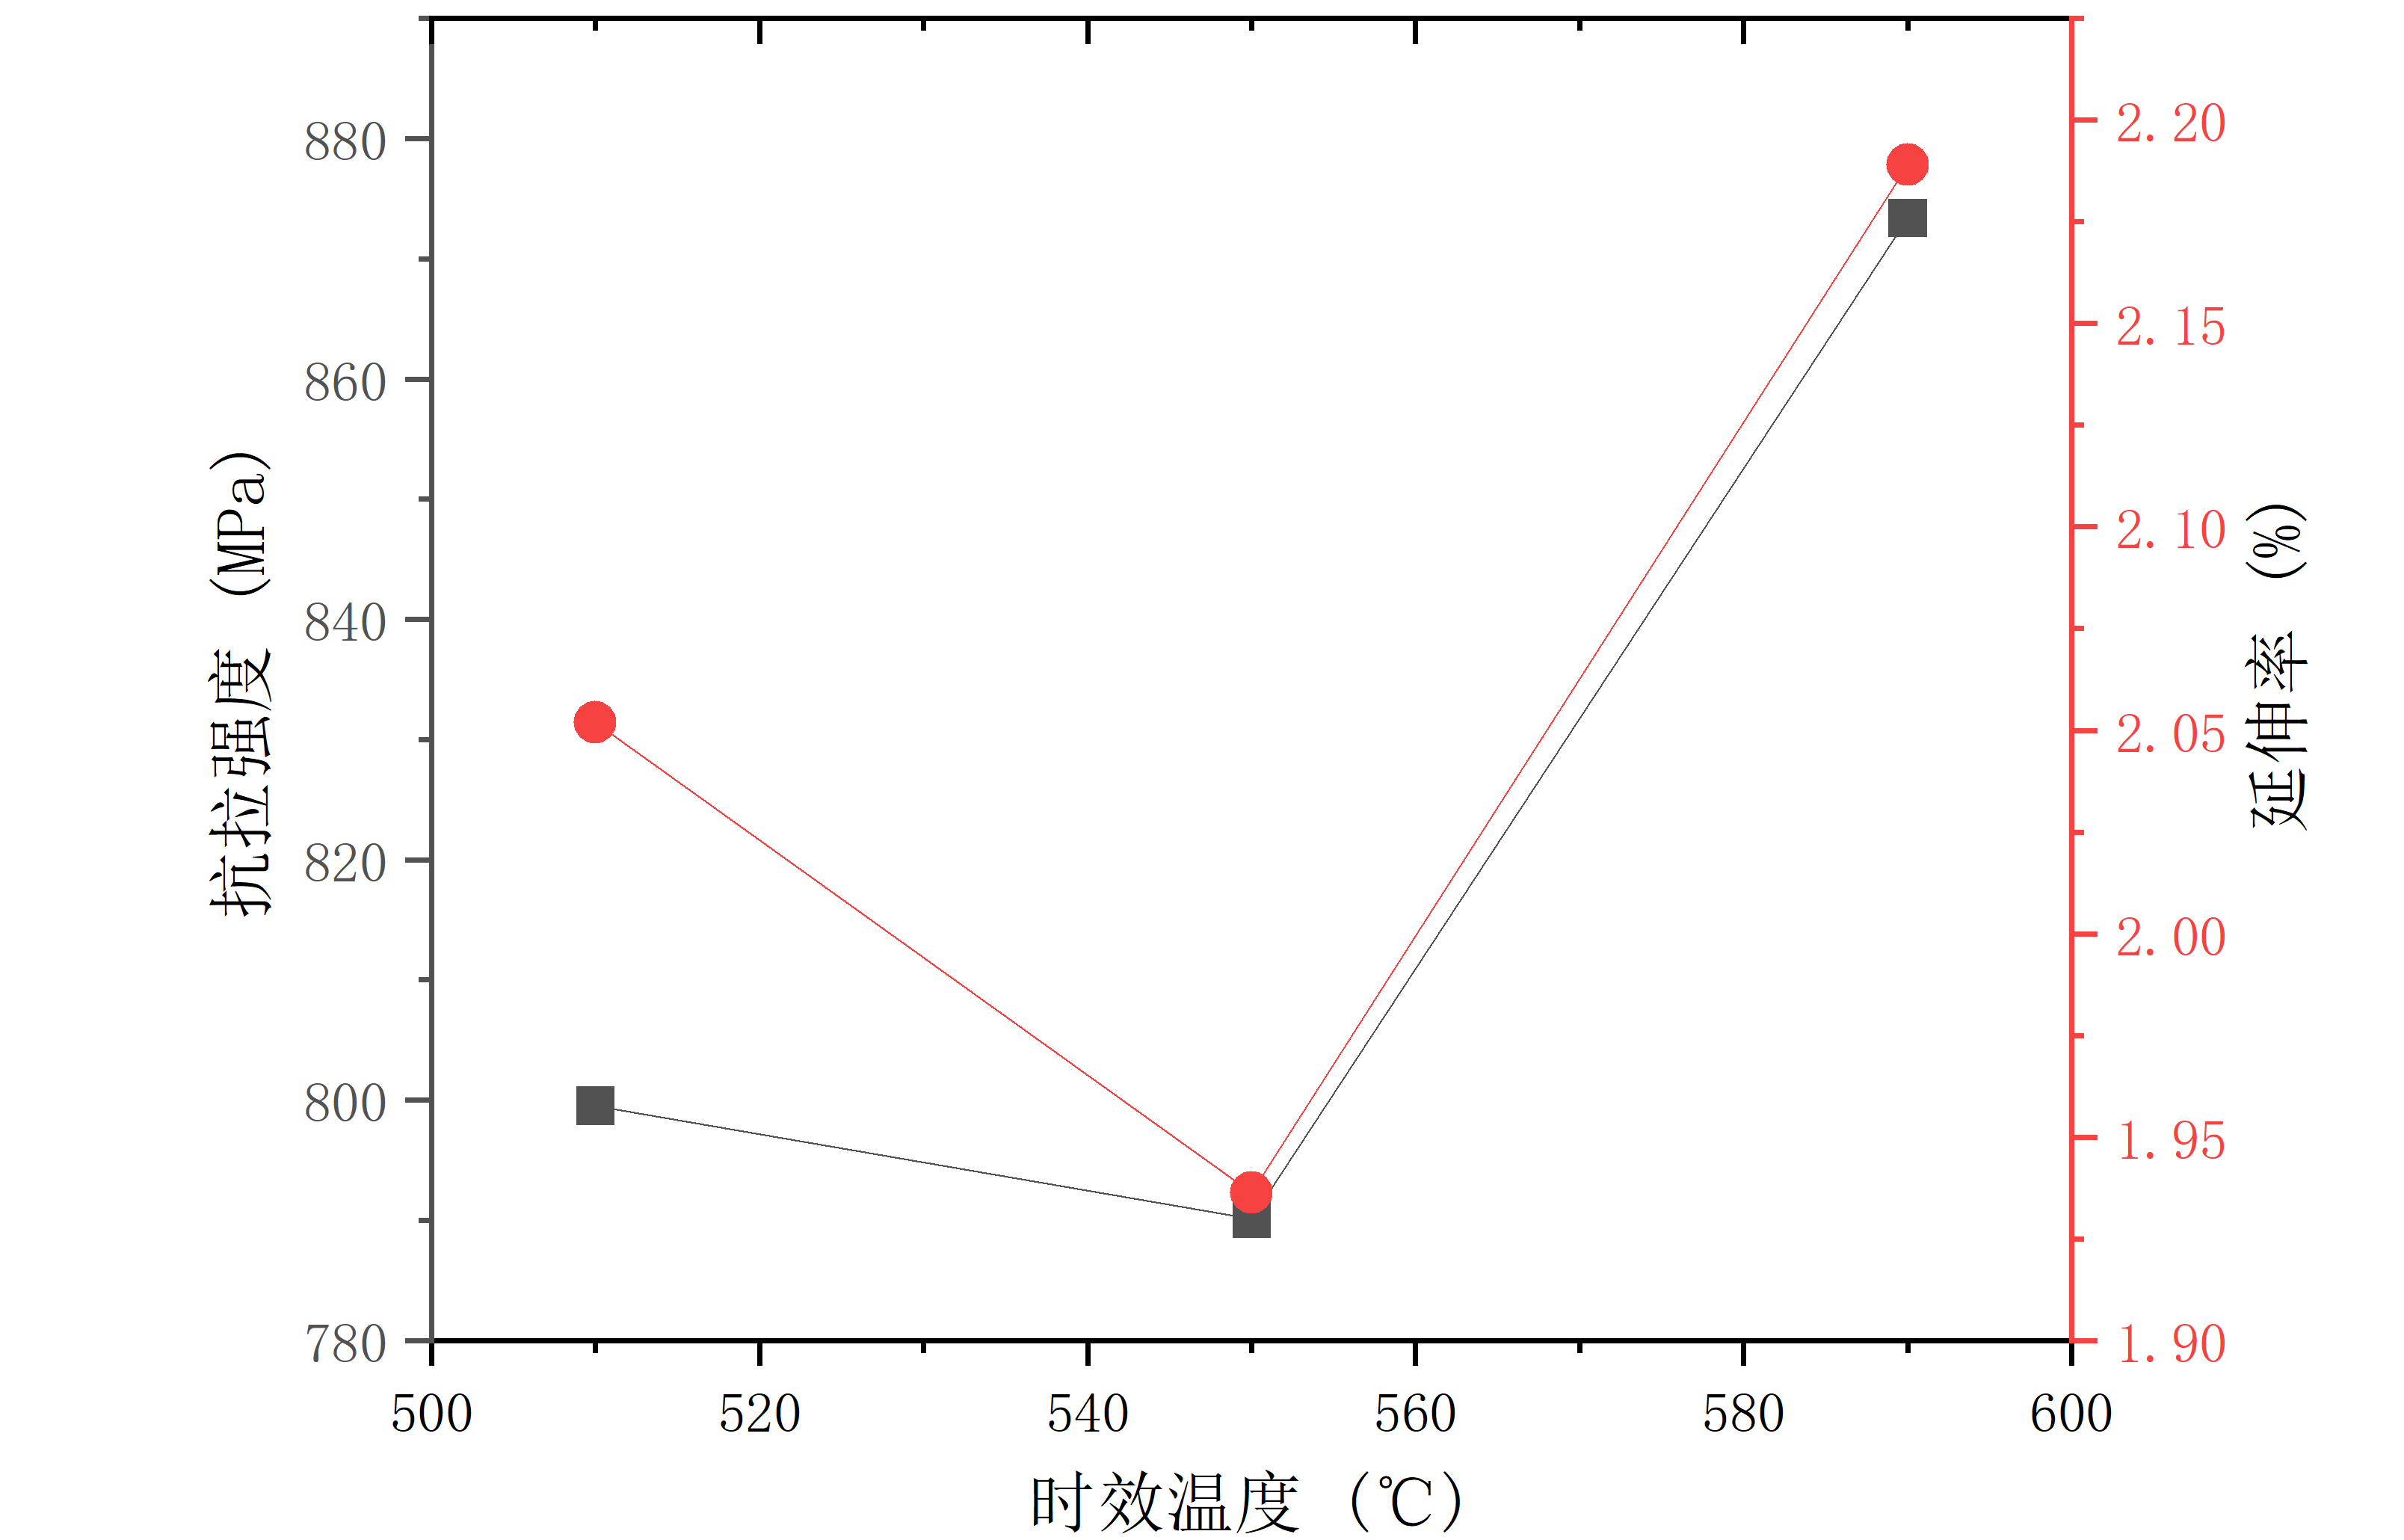
\includegraphics[width=0.7\linewidth]{pic/970分析}
%	\caption{970分析}
%	\label{fig:970}
%\end{figure}



